\documentclass[10pt, letterpaper]{book}

%% packages
\usepackage[utf8]{inputenc}
\usepackage[T1]{fontenc}
\usepackage[spanish, mexico]{babel}
\usepackage{titlesec}
\usepackage{glossaries}
\usepackage{graphicx}

%% page settings
\usepackage[top=2cm, bottom=1.8cm, left=2.5cm, right=2.5cm]{geometry} % for page border settings
\usepackage{fancyhdr} % for head and footer options

%% commands
\newcommand{\tbi}[1]{\textbf{\textit{#1}}}

%% glossary
\makeglossaries
\newglossaryentry{Sucursal}
{
	name={Sucursal},
	description={Sucursal de la Agencia de Renta de Autos.}
}
\newglossaryentry{ModeloAuto}
{
	name={Modelo de Auto},
	description={Modelo del Auto a la renta.}
}

\begin{document}

\title{Requerimientos Funcionales (EU-Car)}
\author{Softtek}
\date{}
\maketitle

\pagestyle{plain}
\tableofcontents

\chapter{Casos de Uso}

%\pagestyle{fancy}
%\fancyhf{}
%\fancyhead[OC]{\leftmark}
%\fancyhead[EC]{\rightmark}
%\cfoot{\thepage}

\section{Modulo: Modelo de Autos}

\subsection{UC05. Crear un Modelo de Auto} \label{CrearModeloAuto}
\textbf{Actores}: Administrador

\textbf{Objetivo}: EU-Rent decide ofrecer a sus Clientes un nuevo modelo de Auto.

\textbf{Evento Disparador}: Administrador solicita la p�gina \textit{[Crear Modelo de Auto]}.

\textbf{Tipo}: Usuario\\

\textbf{Escenario Principal}

\begin{enumerate}
\item El Sistema muestra la p�gina \textit{[Crear Modelo de Auto]}.
\item Administrador captura informaci�n en la forma \textit{[Crear Modelo de Auto]}.
\item Administrador elige el comando \textit{[Guardar]}.
\item El Sistema valida que los datos de la forma \textit{[Crear Modelo de Auto]} estan completos.
	\begin{enumerate}
		\item Excepci�n: Datos incompletos.
	\end{enumerate}
\item El Sistema crea un nuevo registro en la entidad \textit{[ModeloAuto]}.
\item Fin del Caso de Uso.
\end{enumerate}
\subsection{UC06. Buscar un Modelo de Auto} \label{BuscarModeloAuto}
\textbf{Actores}: Administrador

\textbf{Objetivo}: EU-Rent decide buscar un Modelo de Auto para editarlo o eliminarlo.

\textbf{Evento Disparador}: Administrador solicita la p�gina \textit{[Buscar Modelo de Auto]}.

\textbf{Tipo}: Usuario\\

\textbf{Escenario Principal}

\begin{enumerate}
\item El Sistema muestra la p�gina \textit{[Buscar Modelo de Auto]}.
\item Administrador captura informaci�n en la forma \textit{[Criterios de B�squeda]}.
\item Administrador elige el comando \textit{[Buscar]}.
\item El Sistema valida que los datos de la forma \textit{[Criterios de B�squeda]} estan completos.
	\begin{enumerate}
		\item Excepci�n: Datos incompletos.
	\end{enumerate}
\item El Sistema obtiene informaci�n y muestra la lista \textit{[Resultados de B�squeda]}.
\item Fin del Caso de Uso.
\end{enumerate}
\subsection{UC07. Editar un Modelo de Auto} \label{EditarModeloAuto}
\textbf{Actores}: Administrador

\textbf{Objetivo}: EU-Rent decide modificar los datos de un Modelo de Auto.

\textbf{Evento Disparador}: Administrador solicita la p�gina \textit{[Editar Modelo de Auto]}.

\textbf{Tipo}: Usuario\\

\textbf{Escenario Principal}

\begin{enumerate}
\item El Sistema invoca al Caso de Uso \textit{[UC06. Buscar un Modelo de Auto]}.
\item Administrador selecciona el comando \textit{[Editar]}.
\item El Sistema muestra la p�gina \textit{[Editar Modelo de Auto]}.
\item Administrador captura informaci�n en la forma \textit{[Editar Modelo de Auto]}.
\item Administrador elige el comando \textit{[Guardar]}.
\item El Sistema valida que los datos de la forma \textit{[Editar Modelo de Auto]} estan completos.
	\begin{enumerate}
		\item Excepci�n: Datos incompletos.
	\end{enumerate}
\item El Sistema actuliza la informaci�n de la entidad \textit{[ModeloAuto]}.
\item Fin del Caso de Uso.
\end{enumerate}
\subsection{UC08. Eliminar Modelo de Auto} \label{EliminarModeloAuto}
\textbf{Actores}: Administrador

\textbf{Objetivo}: EU Rent decide eliminar un Modelo de Auto existente.

\textbf{Evento Disparador}: Administrador solicita la p�gina \textit{[Eliminar Modelo de Auto]}.

\textbf{Tipo}: Usuario\\

\textbf{Escenario Principal}

\begin{enumerate}
\item El Sistema invoca al Caso de Uso \textit{[UC06. Buscar un Modelo de Auto]}.
\item Administrador selecciona el comando \textit{[Eliminar]}.
\item El Sistema muestra la p�gina \textit{[Eliminar Modelo de Auto]}.
\item Administrador elige el comando \textit{[Eliminar]}.
\item El Sistema elimina el registro de la entidad \textit{[ModeloAuto]}.
\item Fin del Caso de Uso.
\end{enumerate}
\section{Modulo: Sucursales}

\subsection{UC01. Crear una Sucursal} \label{CrearSucursal}
\textbf{Actores}: Administrador

\textbf{Objetivo}: EU-Rent decide abrir una nueva Sucursal.

\textbf{Evento Disparador}: Administrador solicita la p�gina \textit{[Crear Sucursal]}.

\textbf{Tipo}: Usuario\\

\textbf{Escenario Principal}

\begin{enumerate}
\item El Sistema muestra la p�gina \textit{[Crear Sucursal]}.
\item Administrador captura informaci�n en la forma \textit{[Crear Sucursal]}.
\item Administrador elige el comando \textit{[Guardar]}.
\item El Sistema valida que los datos de la forma \textit{[Crear Sucursal]} estan completos.
	\begin{enumerate}
		\item Excepci�n: Datos incompletos.
	\end{enumerate}
\item El Sistema crea un nuevo registro en la entidad \textit{[Sucursal]}.
\item Fin del Caso de Uso.
\end{enumerate}
\subsection{UC02. Buscar una Sucursal} \label{BuscarSucursal}
\textbf{Actores}: Administrador

\textbf{Objetivo}: EU-Rent decide buscar una Sucursal para editarla o eliminarla.

\textbf{Evento Disparador}: Administrador solicita la p�gina \textit{[Buscar Sucursal]}.

\textbf{Tipo}: Usuario\\

\textbf{Escenario Principal}

\begin{enumerate}
\item El Sistema muestra la p�gina \textit{[Buscar Sucursal]}.
\item Administrador captura informaci�n en la forma \textit{[Criterios de B�squeda]}.
\item Administrador elige el comando \textit{[Buscar]}.
\item El Sistema valida que los datos de la forma \textit{[Criterios de B�squeda]} estan completos.
	\begin{enumerate}
		\item Excepci�n: Datos incompletos.
	\end{enumerate}
\item El Sistema obtiene informaci�n y muestra la lista \textit{[Resultados de B�squeda]}.
\item Fin del Caso de Uso.
\end{enumerate}
\subsection{UC03. Editar una Sucursal} \label{EditarSucursal}
\textbf{Actores}: Administrador

\textbf{Objetivo}: EU-Rent decide modificar los datos de una Sucursal.

\textbf{Evento Disparador}: Administrador solicita la p�gina \textit{[Editar Sucursal]}.

\textbf{Tipo}: Usuario\\

\textbf{Escenario Principal}

\begin{enumerate}
\item El Sistema invoca al Caso de Uso \textit{[UC02. Buscar una Sucursal]}.
\item Administrador selecciona el comando \textit{[Editar]}.
\item El Sistema muestra la p�gina \textit{[Editar Sucursal]}.
\item Administrador captura informaci�n en la forma \textit{[Editar Sucursal]}.
\item Administrador elige el comando \textit{[Guardar]}.
\item El Sistema valida que los datos de la forma \textit{[Editar Sucursal]} estan completos.
	\begin{enumerate}
		\item Excepci�n: Datos incompletos.
	\end{enumerate}
\item El Sistema actuliza la informaci�n de la entidad \textit{[Sucursal]}.
\item Fin del Caso de Uso.
\end{enumerate}
\subsection{UC04. Eliminar Sucursal} \label{EliminarSucursal}
\textbf{Actores}: Administrador

\textbf{Objetivo}: EU Rent decide eliminar una Sucursal existente.

\textbf{Evento Disparador}: Administrador solicita la p�gina \textit{[Eliminar Sucursal]}.

\textbf{Tipo}: Usuario\\

\textbf{Escenario Principal}

\begin{enumerate}
\item El Sistema invoca al Caso de Uso \textit{[UC02. Buscar una Sucursal]}.
\item Administrador selecciona el comando \textit{[Eliminar]}.
\item El Sistema muestra la p�gina \textit{[Eliminar Sucursal]}.
\item Administrador elige el comando \textit{[Eliminar]}.
\item El Sistema elimina el registro de la entidad \textit{[Sucursal]}.
\item Fin del Caso de Uso.
\end{enumerate}


\chapter{Especificacion de Interfaz Grafica}

\section{Modulo: Sucursales}

\subsection{Crear Sucursal}

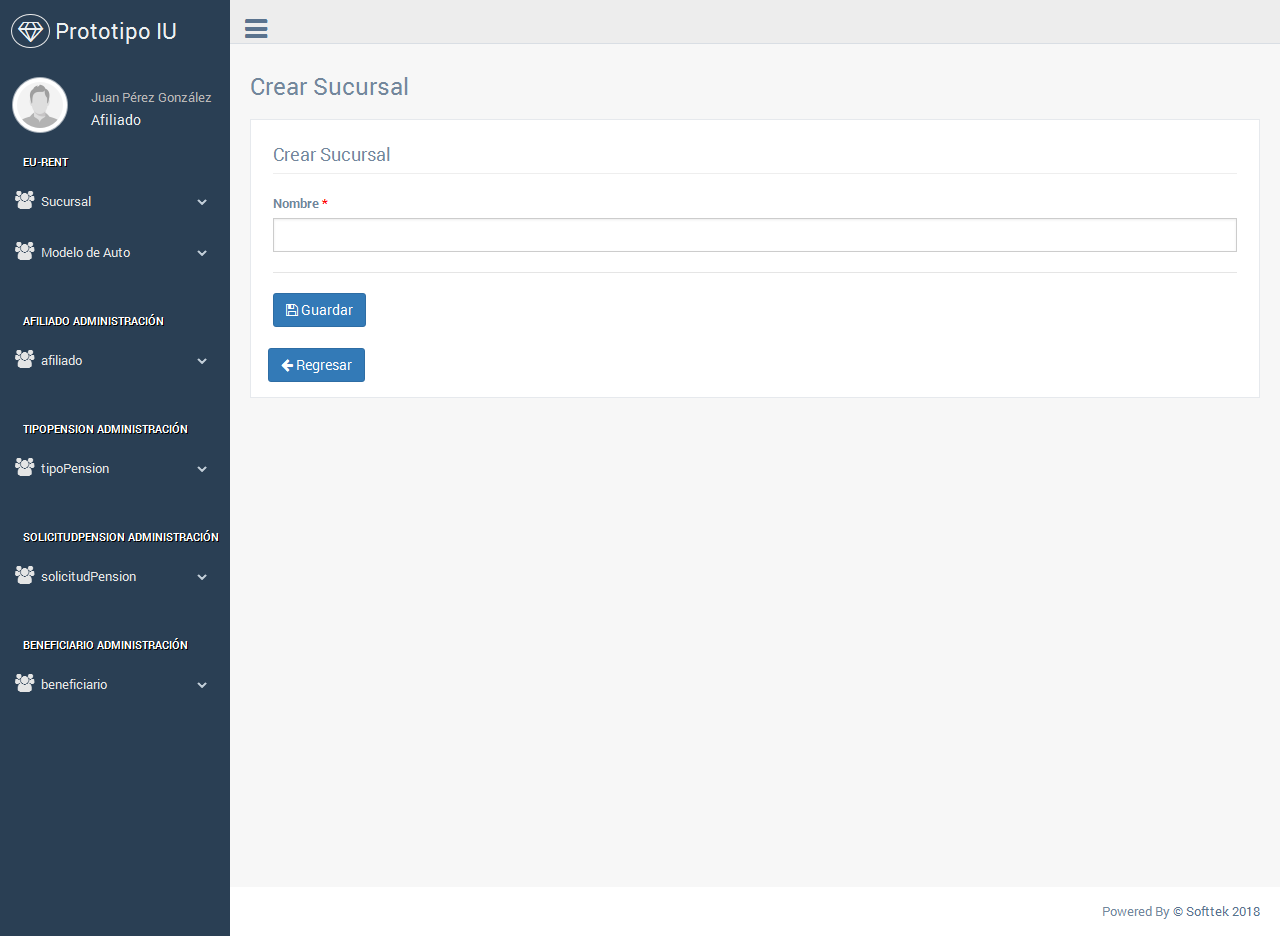
\includegraphics[width=\linewidth]{ui-prototype/SucursalServices/CrearSucursalPage.png}

\begin{center}
 \begin{tabular}{|c c c c|} 
 \hline
 Col1 & Col2 & Col2 & Col3 \\ [0.5ex] 
 \hline\hline
 1 & 6 & 87837 & 787 \\ 
 \hline
 2 & 7 & 78 & 5415 \\
 \hline
 3 & 545 & 778 & 7507 \\
 \hline
 4 & 545 & 18744 & 7560 \\
 \hline
 5 & 88 & 788 & 6344 \\ [1ex] 
 \hline
\end{tabular}
\end{center}



\subsection{Buscar Sucursal}

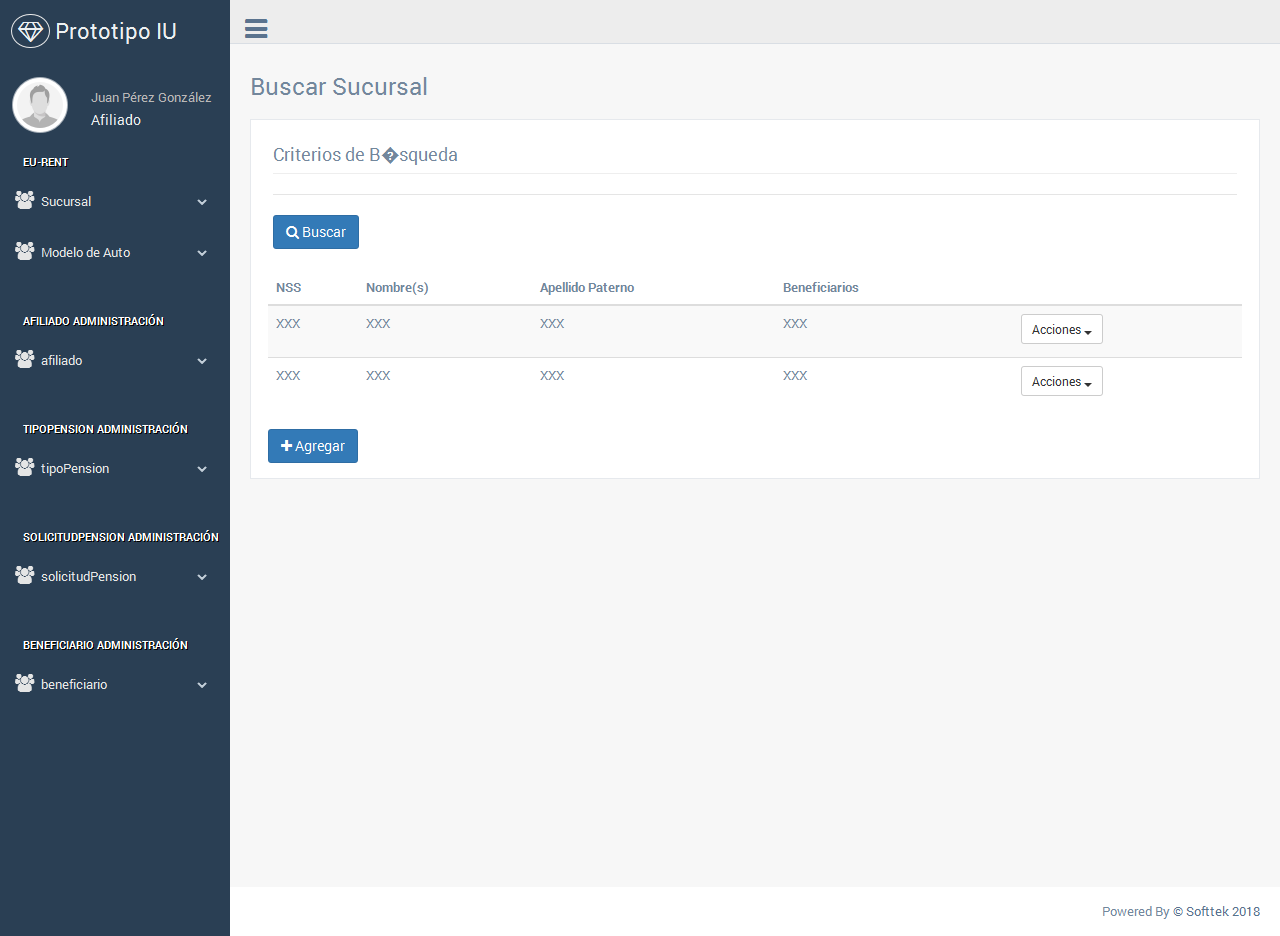
\includegraphics[width=\linewidth]{ui-prototype/SucursalServices/BuscarSucursalPage.png}

\subsection{Editar Sucursal}

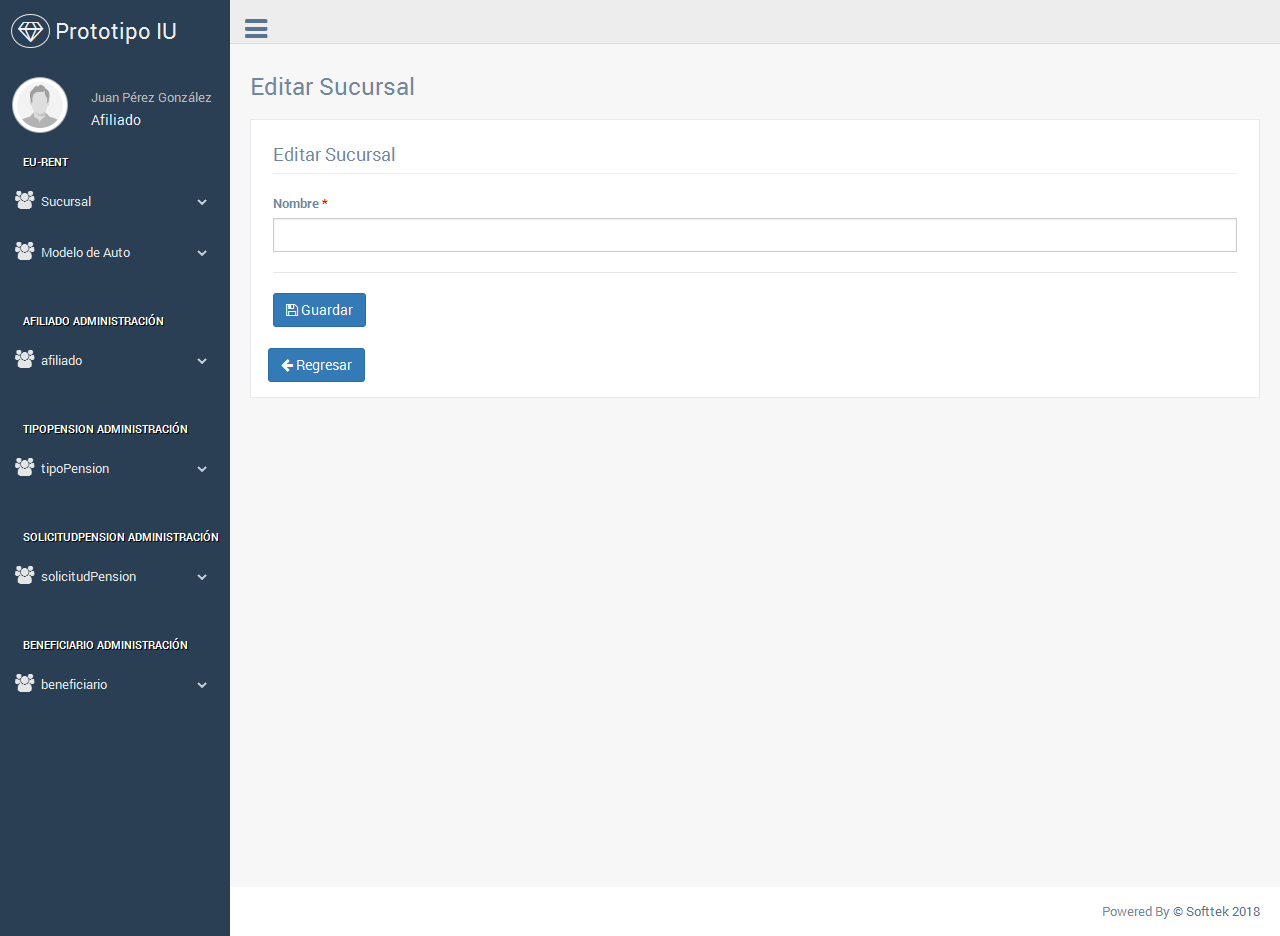
\includegraphics[width=\linewidth]{ui-prototype/SucursalServices/EditarSucursalPage.png}

\subsection{Eliminar Sucursal}

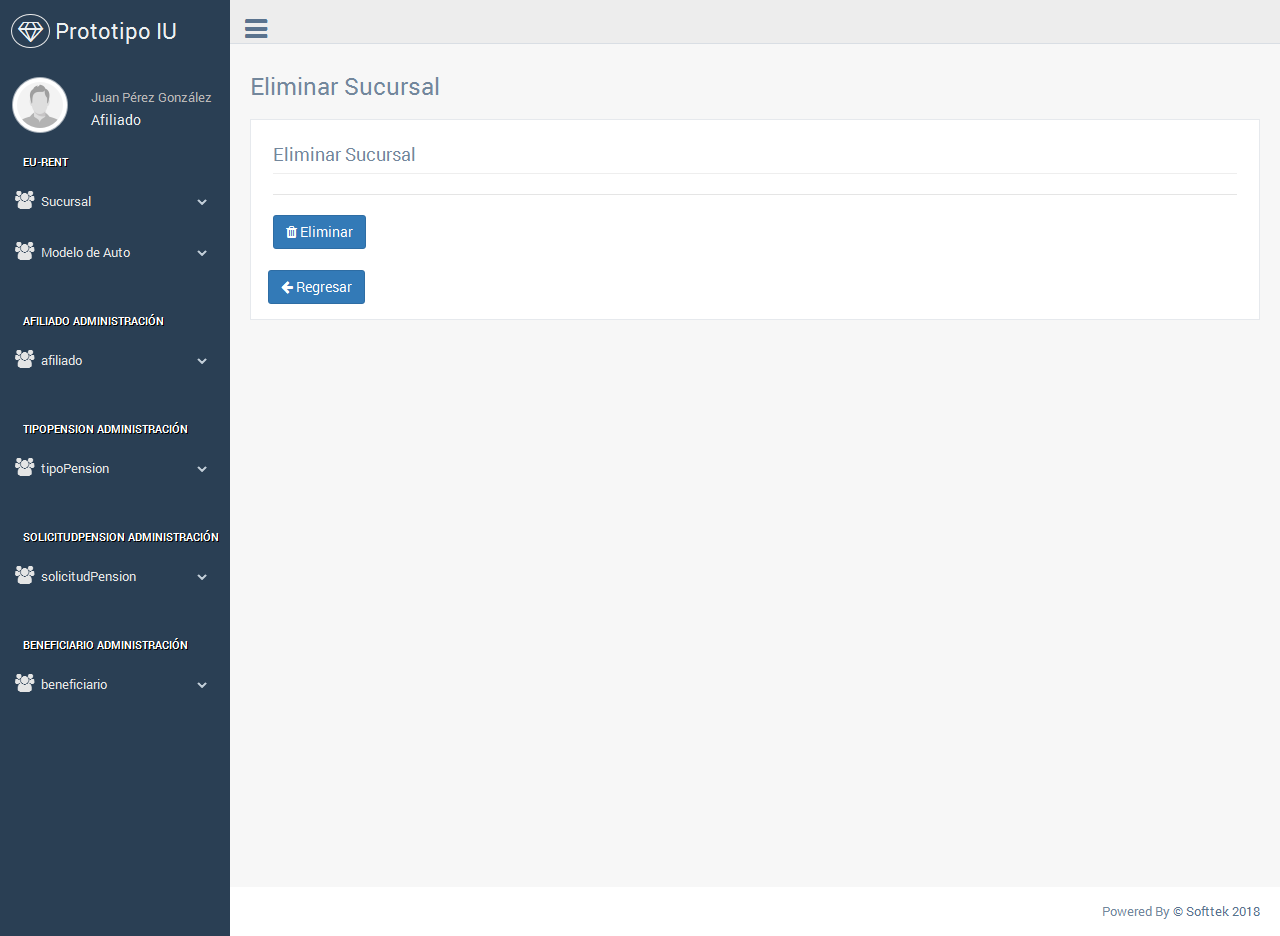
\includegraphics[width=\linewidth]{ui-prototype/SucursalServices/EliminarSucursalPage.png}


\section{Modulo: Modelo de Autos}

\subsection{Crear Modelo de Auto}

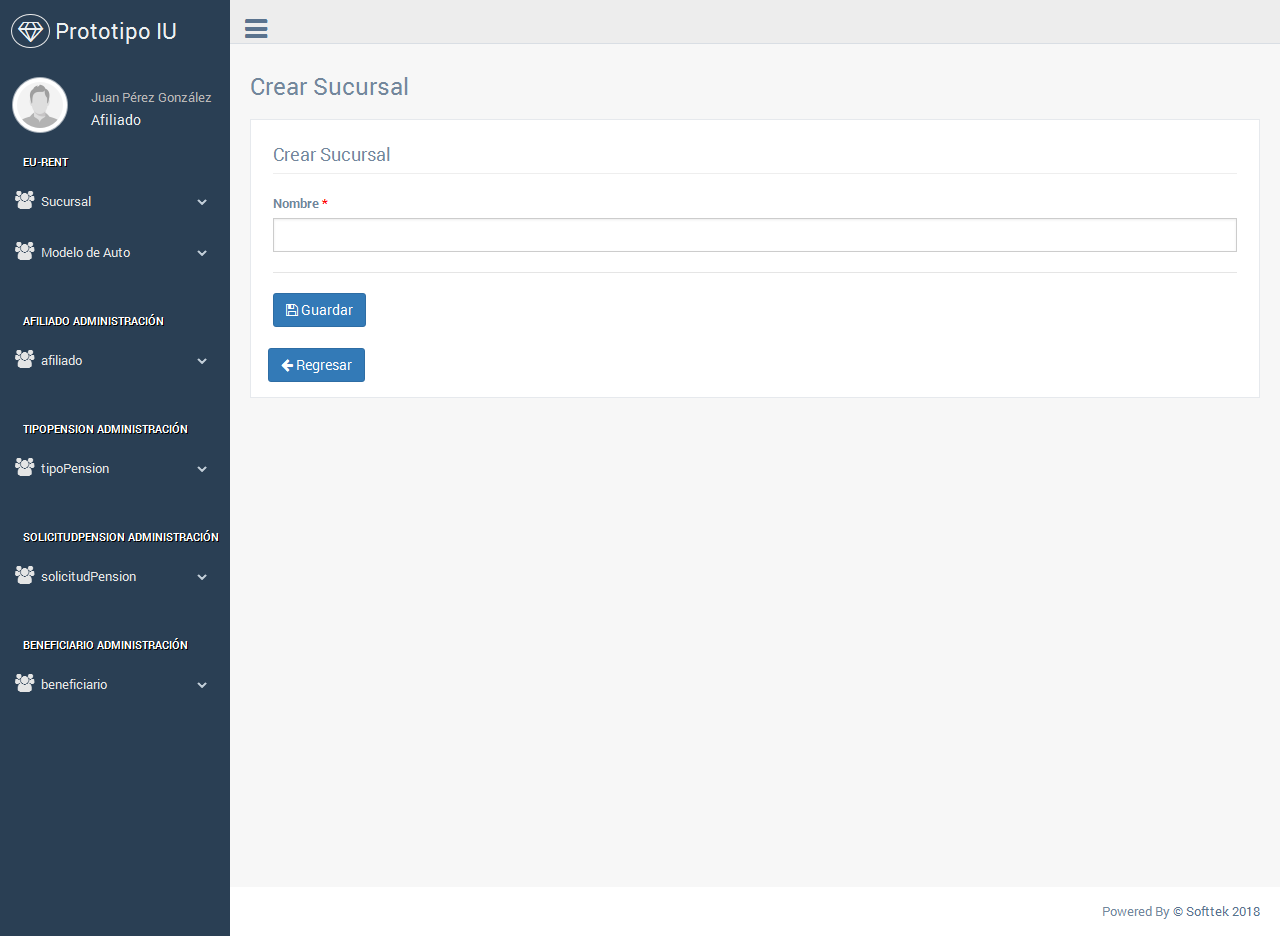
\includegraphics[width=\linewidth]{ui-prototype/SucursalServices/CrearSucursalPage.png}

\subsection{Buscar Modelo de Auto}

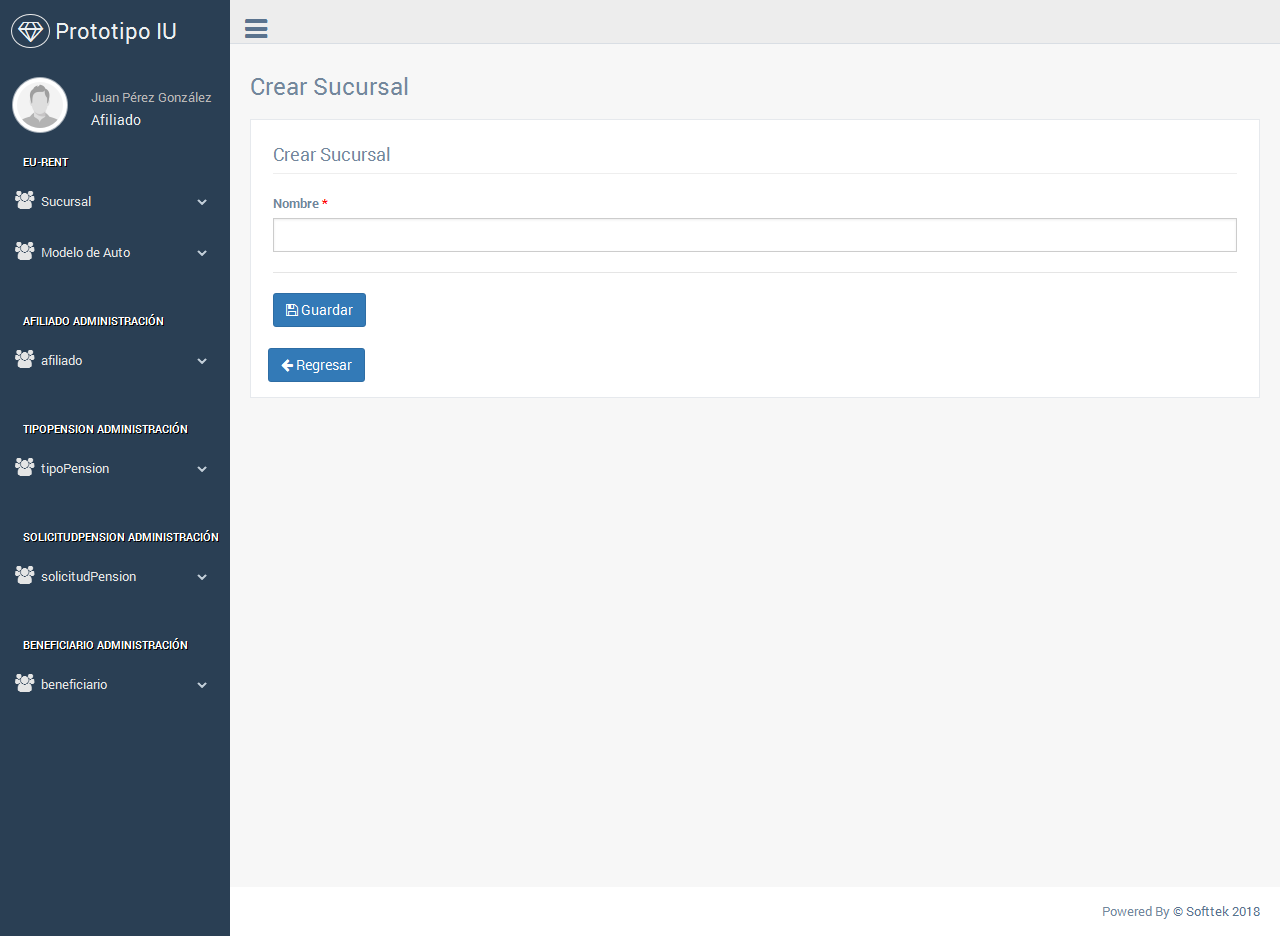
\includegraphics[width=\linewidth]{ui-prototype/SucursalServices/CrearSucursalPage.png}

\subsection{Editar Modelo de Auto}

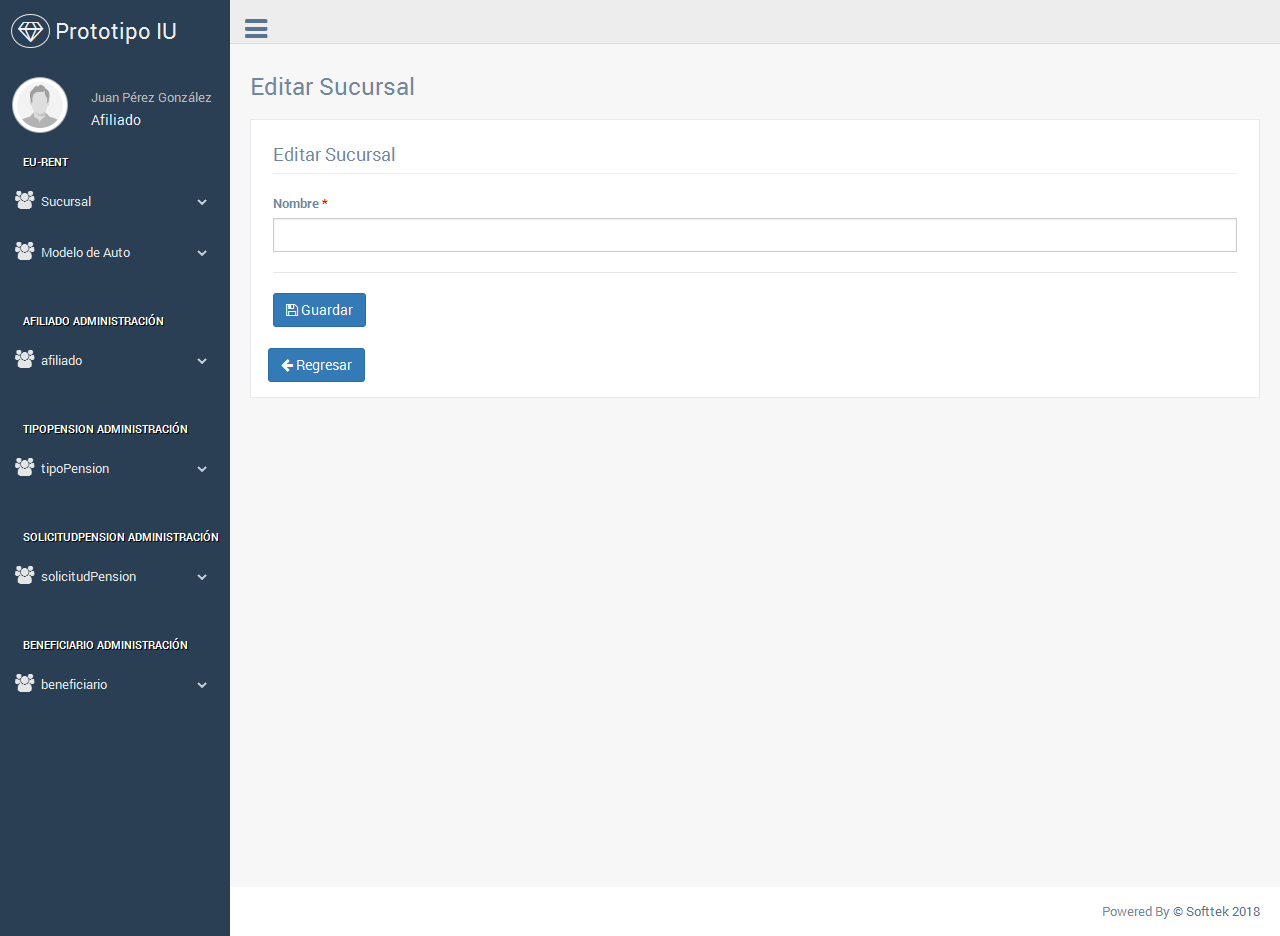
\includegraphics[width=\linewidth]{ui-prototype/SucursalServices/EditarSucursalPage.png}

\subsection{Eliminar Modelo de Auto}

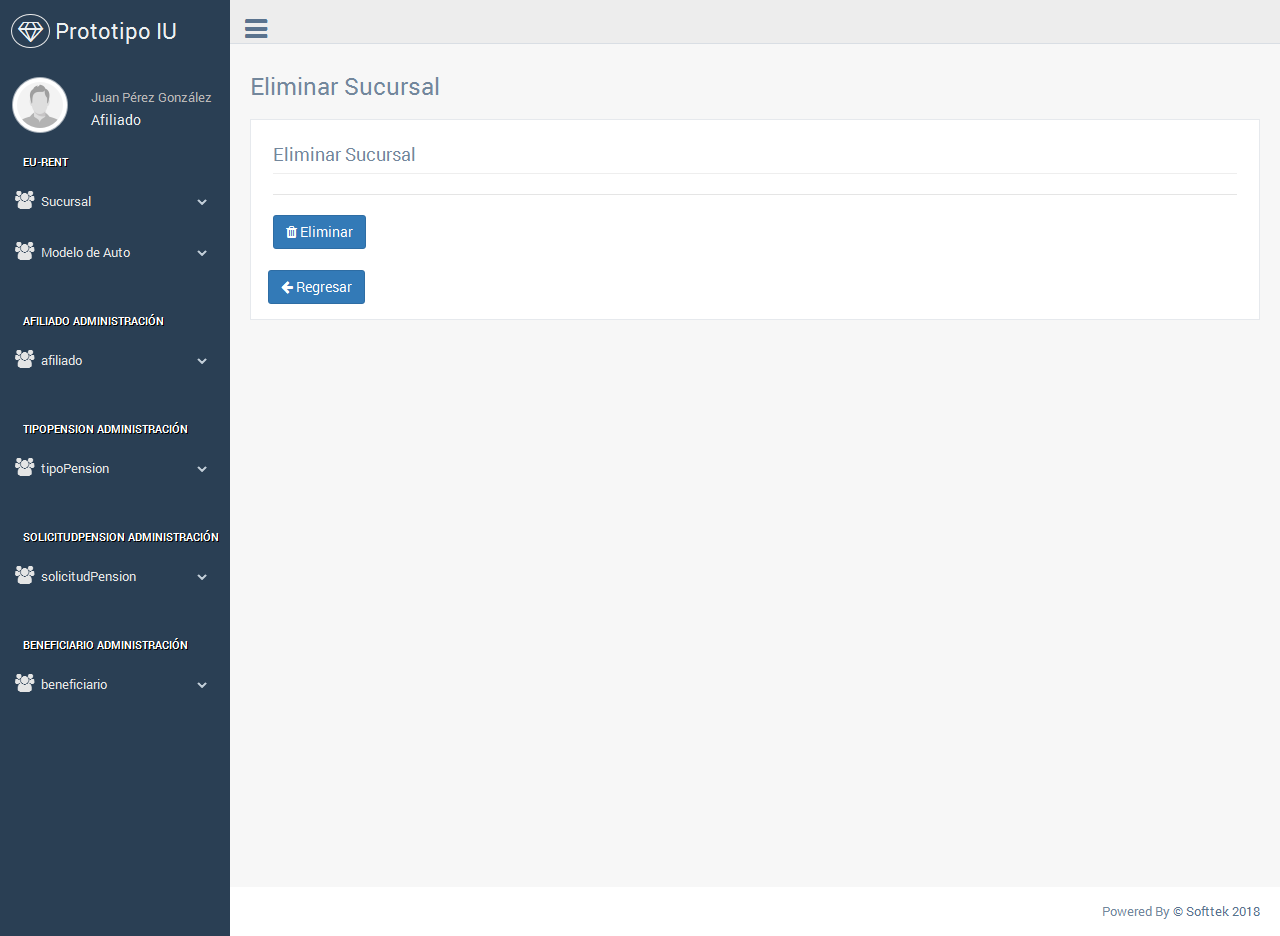
\includegraphics[width=\linewidth]{ui-prototype/SucursalServices/EliminarSucursalPage.png}


%\input{content/pantallas}

\clearpage

\printglossary

\end{document}